%% LyX 2.1.3 created this file.  For more info, see http://www.lyx.org/.
%% Do not edit unless you really know what you are doing.
\documentclass[11pt,english]{article}
\renewcommand{\rmdefault}{cmr}
\renewcommand{\sfdefault}{cmss}
\renewcommand{\ttdefault}{cmtt}
\usepackage[T1]{fontenc}
\usepackage[latin9]{inputenc}
\usepackage{geometry}
\geometry{verbose,tmargin=2.5cm,bmargin=2.5cm,lmargin=2.5cm,rmargin=2.5cm}
\setlength{\parskip}{\bigskipamount}
\setlength{\parindent}{0pt}
\usepackage{babel}
\usepackage{amsthm}
\usepackage{amsmath}
\usepackage{amssymb}
\usepackage{setspace}
\setstretch{0.96}
\usepackage[unicode=true,pdfusetitle,
 bookmarks=true,bookmarksnumbered=false,bookmarksopen=false,
 breaklinks=false,pdfborder={0 0 0},backref=false,colorlinks=false]
 {hyperref}

\makeatletter
%%%%%%%%%%%%%%%%%%%%%%%%%%%%%% Textclass specific LaTeX commands.
\theoremstyle{plain}
\newtheorem{thm}{\protect\theoremname}
  \theoremstyle{plain}
  \newtheorem{cor}[thm]{\protect\corollaryname}
  \theoremstyle{plain}
  \newtheorem{lem}[thm]{\protect\lemmaname}
  \theoremstyle{plain}
  \newtheorem{prop}[thm]{\protect\propositionname}
  \theoremstyle{plain}
  \newtheorem{conjecture}[thm]{\protect\conjecturename}
  \theoremstyle{definition}
  \newtheorem{defn}[thm]{\protect\definitionname}
  \theoremstyle{definition}
  \newtheorem{example}[thm]{\protect\examplename}
  \theoremstyle{remark}
  \newtheorem{rem}[thm]{\protect\remarkname}
  \theoremstyle{remark}
  \newtheorem{claim}[thm]{\protect\claimname}

%%%%%%%%%%%%%%%%%%%%%%%%%%%%%% User specified LaTeX commands.
\date{}

% cleveref allows \ref{thm:asdf} instead of Theorem~\ref{thm:asdf}
\usepackage[nameinlink,capitalise,noabbrev]{cleveref}
\AtBeginDocument{\renewcommand{\ref}[1]{\cref{#1}}}

\usepackage[parfill]{parskip}
\setlength{\parskip}{\bigskipamount}

%have space before theorems
\begingroup
    \makeatletter
    \@for\theoremstyle:=definition,remark,plain\do{%
        \expandafter\g@addto@macro\csname th@\theoremstyle\endcsname{%
            \addtolength\thm@preskip\parskip
            }%
        }
\endgroup

% LyX won't let me include cleveref before theorem declarations so I need to redefine everything as a hack
\theoremstyle{plain}
\newtheorem{mythm}{\protect\theoremname}
\renewenvironment{thm}{\begin{mythm}}{\end{mythm}}
\crefname{mythm}{Theorem}{Theorems}
\theoremstyle{definition}
\newtheorem{mydefn}[mythm]{\protect\definitionname}
\renewenvironment{defn}{\begin{mydefn}}{\end{mydefn}}
\theoremstyle{definition}
\newtheorem{myexample}[mythm]{\protect\examplename}
\renewenvironment{example}{\begin{myexample}}{\end{myexample}}
\theoremstyle{plain}
\newtheorem{myprop}[mythm]{\protect\propositionname}
\renewenvironment{prop}{\begin{myprop}}{\end{myprop}}
\theoremstyle{plain}
\newtheorem{mycor}[mythm]{\protect\corollaryname}
\renewenvironment{cor}{\begin{mycor}}{\end{mycor}}
\theoremstyle{plain}
\newtheorem{mylem}[mythm]{\protect\lemmaname}
\renewenvironment{lem}{\begin{mylem}}{\end{mylem}}
\crefname{mylem}{Lemma}{Lemmas}
\theoremstyle{plain}
\newtheorem{myconjecture}[mythm]{\protect\conjecturename}
\renewenvironment{conjecture}{\begin{myconjecture}}{\end{myconjecture}}
\theoremstyle{remark}
\newtheorem{myrem}[mythm]{\protect\remarkname}
\renewenvironment{rem}{\begin{myrem}}{\end{myrem}}
\theoremstyle{remark}
\newtheorem{myclaim}[mythm]{\protect\claimname}
\renewenvironment{claim}{\begin{myclaim}}{\end{myclaim}}

% equation cref format
\crefformat{equation}{#2(#1)#3}

% \left(\right) should behave the same as ()
\let\originalleft\left
\let\originalright\right
\renewcommand{\left}{\mathopen{}\mathclose\bgroup\originalleft}
\renewcommand{\right}{\aftergroup\egroup\originalright}
\usepackage{pgfplots}
\usetikzlibrary{pgfplots.groupplots}
\usepackage{verbatim}

%make sure tildes in url are vertically centered
\makeatletter
\renewcommand*{\UrlTildeSpecial}{%
  \do\~{%
    \mbox{%
      \fontfamily{ptm}\selectfont
      \textasciitilde
    }%
  }%  
}%    
\let\Url@force@Tilde\UrlTildeSpecial
\makeatother

%graph drawing
\usepackage{tikz}
\usetikzlibrary{external}
\usetikzlibrary{decorations.markings}
\usetikzlibrary{arrows.meta}
\tikzexternalize
\tikzstyle{vertex}=[circle,draw=black,fill=black,inner sep=0,minimum size=0.2cm,text=white,font=\footnotesize]
\tikzset{arc/.style={
        decoration={markings,
            mark= at position 0.5 with {\arrow{Latex[length=2mm,width=2mm]}} ,
        },
        postaction={decorate}
    }
}
\tikzset{every loop/.style={min distance=50,in=50,out=130,looseness=7}}

%caption labels
\usepackage[labelfont=bf,labelsep=period]{caption}

\usepackage{enumitem}

\makeatother

  \providecommand{\claimname}{Claim}
  \providecommand{\conjecturename}{Conjecture}
  \providecommand{\corollaryname}{Corollary}
  \providecommand{\definitionname}{Definition}
  \providecommand{\examplename}{Example}
  \providecommand{\lemmaname}{Lemma}
  \providecommand{\propositionname}{Proposition}
  \providecommand{\remarkname}{Remark}
\providecommand{\theoremname}{Theorem}

\begin{document}

\title{Bounded-degree spanning trees in randomly perturbed graphs}


\author{Michael Krivelevich, Matthew Kwan, Benny Sudakov}

\maketitle
\global\long\def\RR{\mathbb{R}}


\global\long\def\QQ{\mathbb{Q}}


\global\long\def\HH{\mathbb{H}}


\global\long\def\E{\mathbb{E}}


\global\long\def\Var{\operatorname{Var}}


\global\long\def\CC{\mathbb{C}}


\global\long\def\NN{\mathbb{N}}


\global\long\def\ZZ{\mathbb{Z}}


\global\long\def\GG{\mathbb{G}}


\global\long\def\BB{\mathbb{B}}


\global\long\def\DD{\mathbb{D}}


\global\long\def\cL{\mathcal{L}}


\global\long\def\supp{\operatorname{supp}}


\global\long\def\one{\boldsymbol{1}}


\global\long\def\range#1{\left[#1\right]}


\global\long\def\d{\operatorname{d}}


\global\long\def\falling#1#2{\left(#1\right)_{#2}}


\global\long\def\f{\mathbf{f}}


\global\long\def\im{\operatorname{im}}


\global\long\def\sp{\operatorname{span}}


\global\long\def\sign{\operatorname{sign}}


\global\long\def\mod{\operatorname{mod}}


\global\long\def\id{\operatorname{id}}


\global\long\def\disc{\operatorname{disc}}


\global\long\def\lindisc{\operatorname{lindisc}}


\global\long\def\tr{\operatorname{tr}}


\global\long\def\adj{\operatorname{adj}}


\global\long\def\Unif{\operatorname{Unif}}


\global\long\def\Po{\operatorname{Po}}


\global\long\def\Bin{\operatorname{Bin}}


\global\long\def\Ber{\operatorname{Ber}}


\global\long\def\Geom{\operatorname{Geom}}


\global\long\def\Hom{\operatorname{Hom}}


\global\long\def\floor#1{\left\lfloor #1\right\rfloor }


\global\long\def\ceil#1{\left\lceil #1\right\rceil }


\global\long\def\flip#1{\overline{#1}}


\global\long\def\a{\alpha}


\global\long\def\c{c}


\global\long\def\D{\Delta}


\global\long\def\G{G}


\global\long\def\F{F}


\global\long\def\T{T}


\global\long\def\R{R}


\global\long\def\B#1{\Gamma_{A,B}\left(#1\right)}

\begin{abstract}
We show that for any bounded-degree spanning tree $T$ and any fixed
dense graph $G$, a modest random perturbation of $G$ will typically
contain a copy of $T$. This combines the viewpoints of the well-studied
problems of embedding trees into fixed dense graphs and into random
graphs, and extends a sizeable body of existing research on randomly
perturbed graphs. Specifically, we show that there is $\c=\c\left(\a,\D\right)$
such that if $\G$ is an $n$-vertex graph with minimum degree at
least $\a n$, and $\T$ is an $n$-vertex tree with maximum degree
at most $\D$, then if we add $\c n$ uniformly random edges to $\G$,
the resulting graph will contain $\T$ asymptotically almost surely
(as $n\to\infty$). Our proof depends on a lemma concerning the decomposition
of a dense graph into super-regular pairs of uneven sizes, which may
be of independent interest.
\end{abstract}
\begin{comment}
\begin{thm}
t\end{thm}
\begin{cor}
c\end{cor}
\begin{lem}
l\end{lem}
\begin{prop}
p\end{prop}
\begin{conjecture}
c\end{conjecture}
\begin{defn}
d\end{defn}
\begin{example}
e\end{example}
\begin{rem}
r\end{rem}
\begin{claim}
c
\end{claim}
\end{comment}


\section{Introduction}

A classical theorem of Dirac \cite{Dir52} states that any $n$-vertex
graph ($n\ge3$) with minimum degree at least $n/2$ has a Hamilton
cycle: a cycle that passes through all the vertices of the graph.
More recently, there have been many results showing that this kind
of minimum degree condition is sufficient to guarantee the existence
of different kinds of spanning graphs. For example, \cite[Theorem~1$'$]{KSS95}
says that for any $\Delta$ and $\gamma>0$, any $n$-vertex graph
($n$ sufficiently large) with minimum degree $\left(1/2+\gamma\right)n$
contains every spanning tree which has maximum degree at most $\Delta$.
(This has also been generalized further in two directions: to allow
$\Delta$ to grow with $n$ and to allow for much more general spanning
subgraphs than spanning trees; see \cite{KSS01,BST09}).

The constant ``$1/2$'' in the above Dirac-type theorems is tight:
in order to guarantee the existence of these spanning subgraphs we
require very strong density conditions. But the situation is very
different for a ``typical'' large graph. If we fix an arbitrarily
small $\alpha>0$ and select a graph uniformly at random among the
(labelled) graphs with $n$ vertices and $\alpha{n \choose 2}$ edges,
then the degrees will probably each be about $\alpha n$. Such a random
graph is Hamiltonian with probability $1-o\left(1\right)$ (we say
it is Hamiltonian \emph{asymptotically almost surely}, or \emph{a.a.s.}).
This follows from a stronger result \cite{Pos76} that gives a \emph{threshold}
for Hamiltonicity: a random $n$-vertex, $m$-edge graph is Hamiltonian
a.a.s. if $m\gg n\log n$, and fails to be Hamiltonian a.a.s. if $m\ll n\log n$.
Although the exact threshold for bounded-degree spanning trees is
not known, it was proved in \cite{Mon14} that for any $\Delta$ and
any tree $T$ with maximum degree at most $\Delta$, a random $n$-vertex
graph with $\Delta n\left(\log n\right)^{5}$ edges a.a.s. contains
$T$. Here and from now on, all asymptotics are as $n\to\infty$,
and we implicitly round large quantities to integers.

In \cite{BFM03}, the authors studied Hamiltonicity in the random
graph model that starts with a dense graph and adds $m$ random edges.
This model is a natural generalization of the ordinary random graph
model where we start with nothing, and offers a ``hybrid'' perspective
combining the extremal and probabilistic settings of the last two
paragraphs. The model has since been studied in a number of other
contexts; see for example \cite{BHM04,KST06,KKS15}. A property that
holds a.a.s. with small $m$ in our random graph model can be said
to hold not just for a ``globally'' typical graph but for the typical
graph in every small ``neighbourhood'' of our space of graphs. This
tells us that the graphs which fail to satisfy our property are in
some sense ``fragile''. We highlight that it is generally very easy
to transfer results from our model of random perturbation to other
natural models, including those that delete as well as add edges (this
can be accomplished with standard coupling and conditioning arguments).
We also note that a particularly important motivation is the notion
of \emph{smoothed analysis} of algorithms introduced in \cite{ST04}.
This is is a hybrid of worst-case and average-case analysis, studying
the performance of algorithms in the more realistic setting of inputs
that are ``noisy'' but not completely random.

The statement of \cite[Theorem~1]{BFM03} is that for every $\alpha>0$
there is $c=c\left(\alpha\right)$ such that if we start with a graph
with minimum degree at least $\alpha n$ and add $cn$ random edges,
then the resulting graph will a.a.s. be Hamiltonian. This saves a
logarithmic factor over the usual model where we start with nothing.
Note that some dense graphs require a linear number of extra edges
to become Hamiltonian (consider for example the complete bipartite
graph with partition sizes $n/3$ and $2n/3$), so the order of magnitude
of this result is tight.

Let $\GG\left(n,p\right)$ be the Erd\H{o}s-R\'enyi random graph
model with vertex set $\range n=\left\{ 1,\dots,n\right\} $, where
each edge is independently present with probability $p$. (For our
purposes this is equivalent to the model that uniformly at random
selects a $p{n \choose 2}$-edge graph on the vertex set $\range n$).
In this paper we prove the following theorem, extending the aforementioned
result to bounded-degree spanning trees.
\begin{thm}
\label{thm:main-theorem}There is $\c=\c\left(\a,\D\right)$ such
that if $\G$ is a graph on the vertex set $\range n$ with minimum
degree at least $\a n$, and $\T$ is an $n$-vertex tree with maximum
degree at most $\D$, and $\R\in\GG\left(n,\c/n\right)$, then a.a.s.
$\T\subseteq\G\cup\R$.
\end{thm}
One of the ingredients of the proof is the following lemma, due to
Alon and two of the authors (\cite[Theorem~1.1]{AKS07}). It shows
that the random edges in $\R$ are already enough to embed almost-spanning
trees.
\begin{lem}
\label{lem:almost-spanning}There is $\c=\c\left(\varepsilon,\D\right)$
such that $\G\in\GG\left(n,\c/n\right)$ a.a.s. contains every tree
of maximum degree at most $\D$ on $\left(1-\varepsilon\right)n$
vertices.
\end{lem}
We will split the proof of \ref{thm:main-theorem} into two cases
in a similar way to \cite{Kri10}. If our spanning tree $\T$ has
many leaves, then we remove the leaves and embed the resulting non-spanning
tree in $\R$ using \ref{lem:almost-spanning}. To complete this into
our spanning tree $\T$, it remains to match the the vertices needing
leaves with leftover vertices. This amounts to finding a perfect matching
in a certain bipartite graph. The random edges in $\R$ provide several
almost-perfect matchings on their own; we combine these with the dense
graph $\G$ to satisfy the conditions of Hall's marriage theorem and
guarantee the required perfect matching. The details for this case
are given in \ref{sub:many-leaves}.

The more difficult case is where $\T$ has few leaves, which we attack
in \ref{sub:few leaves}. In this case $\T$ cannot be very ``complicated''
and must be a subdivision of a small tree. In particular $\T$ must
have many long \emph{bare paths}: paths where each vertex has degree
exactly two. By removing these bare paths we obtain a small forest
which we can embed into $\R$ using \ref{lem:almost-spanning} (the
details are in \ref{sub:embed-forest}). In order to complete this
forest into our spanning tree $\T$, we need to join up distinguished
pairs of vertices with disjoint paths of certain lengths. In order
to make this task feasible, in \ref{sub:partition-into-blobs} we
first use Szemer\'edi's regularity lemma to divide the vertex set
into a bounded number of pieces, each of which induces a ``super-regular
pair'' in $\G$ (that is, a dense subgraph with edges very well-distributed).
In \ref{sub:embed-paths-between} we use $\R$ to find most of our
desired paths, in such a way that it only remains to join up pairs
of vertices within the same super-regular pair. We make some further
adjustments with $\R$ (\ref{sub:embed-relative-sizes}), after which
the super-regularity of the pairs allows us to find the rest of our
paths using a tool called the ``blow-up lemma'' (\ref{sub:blow-up}).


\section{Proof of \texorpdfstring{}{Theorem~}\ref{thm:main-theorem}}

We split the random edges into multiple independent ``phases'':
say $\R\supseteq\R_{1}\cup\R_{2}\cup\R_{3}\cup\R_{4}$, where $\R_{i}\in\GG\left(n,\c_{i}/n\right)$
for some large $\c_{i}=\c_{i}\left(\a,\D\right)$ to be determined
later (these $\c_{i}$ will in turn determine $\c$). Let $V=\range n$
be the common vertex set of $\G$, $\R$ and the $\R_{i}$.

At several points in the proof we will prove that (with high probability)
there exist certain substructures in the random edges $\R$, and we
will assume that these substructures (or some corresponding vertex
sets) are themselves uniformly random. A simple way to see why this
kind of reasoning is valid, is to notice that if we apply a uniformly
random vertex permutation to a random graph $\R\in\GG\left(n,p\right)$,
then by symmetry the resulting distribution is still $\GG\left(n,p\right)$.
So we can imagine that we are finding substructures in an auxiliary
random graph, then randomly mapping these structures to our vertex
set.


\subsection{Case 1: $\protect\T$ has many leaves\label{sub:many-leaves}}

For our first case suppose there are at least $\lambda n$ leaves
in $\T$ (for some fixed $\lambda=\lambda\left(\a\right)>0$ to be
determined in the second case). Then consider the tree $\T'$ with
some $\lambda n$ leaves removed. By \ref{lem:almost-spanning} we
can a.a.s. embed $\T'$ into $\R_{1}$. Let $A'\subseteq V$ be the
set of vertices of $\T'$ which had a leaf deleted from them, and
let $B\subseteq V$ be the set of $\lambda n$ vertices not part of
$\T'$. We can assume $A'$ and $B$ are uniformly random disjoint
sets of the appropriate size (note $\left|A'\right|\ge\lambda n/\D$
and $\left|B\right|=\lambda n$). For each $a\in A'$, the random
variable $\left|N_{\G}\left(a\right)\cap B\right|$ is hypergeometrically
distributed with expected value $\lambda\a n$, and similarly each
$\left|N_{\G}\left(b\right)\cap A'\right|$ ($b\in B$) is hypergeometric
with expectation at least $\lambda\a n/\D$. Let $\beta=\lambda\a/\left(2\D\right)$;
by a concentration inequality (for example, see \cite[Theorem 2.10]{JLR00})
and the union bound, in $\G$ each $a'\in A'$ a.a.s. has at least
$\beta n$ neighbours in $B$, and each $b\in B$ a.a.s. has at least
$\beta n$ neighbours in $A'$. From now on we treat $A'$ and $B$
as fixed sets satisfying these properties.

Let $A$ be a set consisting of $\ell$ copies of each vertex $a'\in A'$
which needs $\ell$ extra leaves (so $\left|A\right|=\lambda n$).
Define a bipartite graph $\B{\G}$ on the vertex set $A\cup B$, with
an edge between $a\in A$ (a copy of $a'\in A'$) and $b\in B$, if
there is an edge between $a'$ and $b$ in $\G$. Similarly define
$\B{\R_{2}}$ and $\B{\G\cup\R}$ with edges deriving from $\R_{2}$
and $\G\cup\R$. If we can find a perfect matching in $\B{\G}\cup\B{\R_{2}}\subseteq\B{\G\cup\R}$,
this gives us a way to extend our embedding of $\T'$ to an embedding
of $\T$, as desired.

Let $\BB_{A,B}\left(p\right)$ be the random bipartite graph distribution
where each of the $\left|A\right|\left|B\right|$ possible edges between
$A$ and $B$ are present with probability $p$. For any $\c_{\BB}$,
we can choose large $\c_{2}$ such that for any $a'\in A$ and $b\in B$,
and for large $n$, 
\begin{align*}
 & \Pr\left(\mbox{all copies of }a'\mbox{ are adjacent to }b\mbox{ in }\B{\R_{2}}\right)=\c_{2}/n\\
 & \quad\ge1-\left(1-\c_{\BB}/n\right)^{\Delta}=\Pr\left(\mbox{some copy of }a'\mbox{ is adjacent to }b\mbox{ in }\BB_{A,B}\left(\c_{\BB}/n\right)\right).
\end{align*}
This means we can couple $\B{\R_{2}}$ and $G_{\BB}\in\BB_{A,B}\left(\c_{\BB}/n\right)$
in such a way that $\B{\R_{2}}\supseteq G_{\BB}$ (the distribution
of $\B{\R_{2}}$ \emph{stochastically dominates} $\BB_{A,B}\left(\c_{\BB}/n\right)$).
The following lemma then provides the desired perfect matching.
\begin{lem}
\label{lem:bipartite-perfect-matching}Let $A$ and $B$ be $n$-vertex
sets. There is $\c_{\BB}=\c_{\BB}\left(\a\right)$ such that if $\G$
is a bipartite graph with bipartition $A\cup B$ and minimum degree
at least $\a n$, and if $\R\in\BB_{A,B}\left(\c_{\BB}/n\right)$,
then a.a.s. $\G\cup\R$ has a perfect matching.
\end{lem}
In order to prove \ref{lem:bipartite-perfect-matching} we need another
lemma.
\begin{lem}
\label{lem:bipartite-matching}Let $\varepsilon>0$, and let $A$
and $B$ be $n$-vertex sets. There is $\c=\c\left(\varepsilon\right)$
such that $\R\in\BB_{A,B}\left(\c/n\right)$ has a matching of size
$\left(1-\varepsilon\right)n$.\end{lem}
\begin{proof}
For any subsets $A'$ and $B'$ of size $\varepsilon n$, the probability
there is no edge between $A'$ and $B'$ is $\left(1-\c/n\right)^{\left(\varepsilon n\right)^{2}}\le e^{-\c\varepsilon^{2}n}$.
There are at most $2^{2n}$ choices of such $A',B'$, so for large
$\c$, by the union bound there is a.a.s. an edge between any such
pair of sets. It follows that a maximum-size matching a.a.s. has at
least $\left(1-\varepsilon\right)n$ edges.
\end{proof}

\begin{proof}[Proof of \ref{lem:bipartite-perfect-matching}]
We apply Hall's marriage theorem. If $W\subseteq A$ with $\left|W\right|\le\a n$
then $\left|N_{\G}\left(W\right)\right|\ge\a n\ge\left|W\right|$
by the minimum degree condition on $\G$. Similarly, every vertex
outside $N_{\G}\left(W\right)$ has at least $\a n$ neighbours outside
$W$, so if $\left|W\right|\ge\left(1-\a\right)n$ then $\left|N_{\G}\left(W\right)\right|=n\ge\left|W\right|$.
So, consider any $W$ with $\a n\le\left|W\right|\le\left(1-\a\right)n$
(in which case we must have $\a\le1/2$). Split $\R$ into phases
$\R\supseteq\R_{1}\cup\dots\cup\R_{r}$, with $\R_{i}\in\BB_{A,B}\left(\c'/n\right)$,
for some $\c'=\c'\left(\a\right)$ and $r=r\left(\a\right)$ to be
determined.

By \ref{lem:bipartite-matching}, if $\c'$ is large we can find a
$\left(1-\a/8\right)n$-edge matching $M_{i}$ in each $\R_{i}$.
Let $N_{i}=N_{M_{i}}\left(W\right)$ contain the vertices matched
with $W$ in each $M_{i}$, and note that each $N_{i}$ is a random
set satisfying $\left|W\right|-\a n/8\le\left|N_{i}\right|\le\left|W\right|$.
Condition on $N_{1}$, and condition on the number of vertices $\left|N_{i}\right|$
matched by $W$ in each $M_{i}$. Now, for each $i>1$, note that
$\left|N_{i}\cap N_{1}\right|$ is hypergeometrically distributed
with mean $\left|N_{i}\right|\left|N_{1}\right|/n$. Since $\left|W\right|\left(n-\left|W\right|\right)\ge\a n\left(1-\a\right)n\ge\a n^{2}/2$,
we have $\left|W\right|^{2}\le\left|W\right|n-\a n^{2}/2$ and 
\[
\left|N_{i}\right|\left|N_{1}\right|/n\le\left|W\right|^{2}/n\le\left|W\right|-\a n/2=2\left(\left|W\right|-\a/8\right)-\left|W\right|-\a/4\le\left|N_{i}\right|+\left|N_{1}\right|-\left|W\right|-\a n/4.
\]
So, by a concentration inequality,
\[
\Pr\left(\left|N_{i}\cup N_{1}\right|<\left|W\right|\right)=\Pr\left(\left|N_{i}\cap N_{1}\right|>\left|N_{i}\right|+\left|N_{1}\right|-\left|W\right|\right)=e^{-\Omega\left(\a^{2}n\right)}
\]
and therefore
\[
\Pr\left(\left|N_{\R}\left(W\right)\right|<\left|W\right|\right)\le\prod_{i=2}^{r}\Pr\left(\left|N_{i}\cup N_{1}\right|<\left|W\right|\right)=e^{-\Omega\left(r\a^{2}n\right)}.
\]
If $r$ is large this probability is $o\left(2^{-n}\right)$, and
since there are at most $2^{n}$ choices for $W$, the union bound
gives $\left|N_{\R}\left(W\right)\right|\ge\left|W\right|$ for all
required $W$.
\end{proof}

\subsection{Case 2: $\protect\T$ has few leaves\label{sub:few leaves}}

Now we address the second case where there are fewer than $\lambda n$
leaves in $\T$.


\subsubsection{Partitioning into super-regular pairs\label{sub:partition-into-blobs}}

As outlined, we first need to divide $G$ into a bounded number of
pairs of clusters with edges well-distributed between them. This partition
will inform the way we use $\R$ to embed $\T$.

\global\long\def\h{h}

\begin{defn}
For a disjoint pair of vertex sets $\left(X,Y\right)$ in a graph,
let its \emph{density} $d\left(X,Y\right)$ be the number of edges
between $X$ and $Y$, divided by $\left|X\right|\left|Y\right|$.
A pair of vertex sets $\left(V_{1},V_{2}\right)$ is said to be \emph{$\varepsilon$-regular}
if for any $U_{1},U_{2}$ with $U_{\h}\subseteq V_{\h}$ and $\left|U_{\h}\right|\ge\varepsilon\left|V_{\h}\right|$,
we have $\left|d\left(U_{1},U_{2}\right)-d\left(V_{1},V_{2}\right)\right|\le\varepsilon$.
If alternatively $d\left(U_{1},U_{2}\right)\ge\delta$ for all such
pairs $U_{1},U_{2}$ then we say $\left(V_{1},V_{2}\right)$ is \emph{$\left(\varepsilon,\delta\right)$-dense}.
Let $\flip{\h}=2-\h$; if $\left(V_{1},V_{2}\right)$ is $\left(\varepsilon,\delta\right)$-dense
and moreover each $v\in V_{\h}$ has at least $\delta\left|V_{\flip{\h}}\right|$
neighbours in $V_{\flip{\h}}$, then we say $\left(V_{1},V_{2}\right)$
is \emph{$\left(\varepsilon,\delta\right)$-super-regular}.\end{defn}
\begin{lem}
\label{lem:partition-into-blobs}For $\a,\varepsilon>0$ with $\varepsilon$
sufficiently small relative to $\a$, there are $\delta=\delta\left(\a\right)>0$
and $M=M\left(\a,\varepsilon\right)$, such that the following holds.
Let $\G$ be a graph on $\range n$ with minimum degree at least $\a n$.
We can choose $q\le M$ and partition $\range n$ into sets $V_{i}^{\h}$
($1\le i\le q$, $\h=1,2$) such that each $\left|V_{i}^{\h}\right|=\Theta\left(n\right)$
and each pair $\left(V_{i}^{1},V_{i}^{2}\right)$ is $\left(\varepsilon,\delta\right)$-super-regular.
\end{lem}
We emphasize that in \ref{lem:partition-into-blobs} we do \emph{not
}guarantee that the sets $V_{i}^{\h}$ are the same size. We will
however see in the proof that the variation in the sizes of the clusters
only depends on $\a$ and not $\varepsilon$ (that is, the ratio between
the largest and smallest cluster is bounded by a function of $\a$).

To prove \ref{lem:partition-into-blobs}, we will apply Szemer\'edi's
regularity lemma to obtain a reduced \emph{cluster graph}, then decompose
this cluster graph into small stars. In each star $T_{i}$, the centre
cluster will correspond to $V_{i}^{1}$ and the leaf clusters will
be combined to form $V_{i}^{2}$. We will then have to redistribute
some of the vertices to ensure super-regularity. Before giving the
details of the proof, we give a statement of (a version of) Szemer\'edi's
regularity lemma and some auxiliary lemmas for working with regularity
and super-regularity.
\begin{lem}[Szemer\'edi's regularity lemma, minimum degree form]
\label{lem:szemeredi-regularity}For every $\a>0$, and any $\varepsilon>0$
that is sufficiently small relative to $\a$, there is $\a'=\a'\left(\a\right)>0$
and $K=K\left(\varepsilon\right)$ such that the following holds.
For any graph $\G$ of minimum degree at least $\a\left|\G\right|$,
there is a partition of $V\left(\G\right)$ into clusters $V_{0},V_{1},\dots V_{k}$
($k\le K$), and a spanning subgraph $\G'$ of $\G$, satisfying the
following properties. The ``exceptional cluster'' $V_{0}$ has size
at most $\varepsilon n$, and the other clusters have equal size $sn$.
The minimum degree of $\G'$ is at least $\a'n$. There are no edges
of $\G'$ within clusters, and each pair of non-exceptional clusters
is $\varepsilon$-regular in $\G'$ with density zero or at least
$\a'$. Moreover, define the \emph{cluster graph} $C$ as the graph
whose vertices are the $k$ non-exceptional clusters $V_{i}$, and
whose edges are the pairs of clusters between which there is nonzero
density in $\G'$. The minimum degree of $C$ is at least $\a'k$.
\end{lem}
This version of Szemeredi's regularity lemma follows directly from
\cite[Proposition~9]{KOT05}.

Before we proceed to the proof of \ref{lem:partition-into-blobs},
we give some simple lemmas about $\left(\varepsilon,\delta\right)$-denseness.
Note that $\left(\varepsilon,\delta\right)$-denseness is basically
a one-sided version of $\varepsilon$-regularity that is more convenient
in proofs about super-regularity. Here and in later sections, most
of the theorems about $\left(\varepsilon,\delta\right)$-dense pairs
correspond to analogous theorems for $\varepsilon$-regular pairs
with density about $\delta$.
\begin{lem}
\label{lem:combine-clusters}Suppose $V_{1}^{2},\dots,V_{r}^{2}$
are clusters such that each $\left(V^{1},V_{i}^{2}\right)$ is $\left(\varepsilon,\delta\right)$-dense.
Let $V^{2}=\bigcup_{i=1}^{r}V_{i}^{2}$; then $\left(V^{1},V^{2}\right)$
is $\left(\varepsilon,\delta'\right)$-dense, where $\delta'=\delta\min_{i}\left|V_{i}^{2}\right|/\left|V^{2}\right|$.
In particular if each $V_{i}^{2}$ has the same size then $\delta'=\delta/r$.
If moreover each each $\left(V^{1},V_{i}^{2}\right)$ is $\left(\varepsilon,\delta\right)$-super-regular,
then $\left(V^{1},V^{2}\right)$ is $\left(\varepsilon,\delta'\right)$-super-regular.\end{lem}
\begin{proof}
Let $U^{\h}\subseteq V^{\h}$ with $\left|U^{\h}\right|\ge\varepsilon\left|V^{\h}\right|$.
Choose $i$ so that $\left|U^{2}\cap V_{i}^{2}\right|/\left|V_{i}^{2}\right|$
is maximized, so that $\left|U^{2}\cap V_{i}^{2}\right|\ge\varepsilon\left|V_{i}^{2}\right|$.
By our choice of $i$, 
\[
\left|U^{2}\right|=\sum_{j=1}^{r}\frac{\left|U^{2}\cap V_{j}^{2}\right|}{\left|V_{j}^{2}\right|}\left|V_{j}^{2}\right|\le\frac{\left|U^{2}\cap V_{i}^{2}\right|}{\left|V_{i}^{2}\right|}\sum_{j=1}^{r}\left|V_{j}^{2}\right|=\frac{\left|U^{2}\cap V_{i}^{2}\right|}{\left|V_{i}^{2}\right|}\left|V^{2}\right|,
\]
so $\left|U^{2}\cap V_{i}^{2}\right|\ge\left|U^{2}\right|\min_{j}\left|V_{j}^{2}\right|/\left|V^{2}\right|$.
It follows that there are at least $\delta\left|U^{1}\right|\left|U^{2}\cap V_{i}^{2}\right|\ge\delta'\left|U^{1}\right|\left|U^{2}\right|$
edges between $U^{1}$ and $U^{2}$, and $\left(V^{1},V^{2}\right)$
is $\left(\varepsilon,\delta'\right)$-dense.

The claim about super-regularity is straightforward. Note that each
$v\in V^{2}$ has $\delta\left|V^{1}\right|\ge\delta'\left|V^{1}\right|$
neighbours in $V^{1}$ by the super-regularity of each $\left(V^{1},V_{i}^{2}\right)$.
Each $v\in V^{1}$ has $\delta\left|V_{i}^{2}\right|$ neighbours
in each $V_{i}^{1}$, for a total of $\delta\left|V^{2}\right|\ge\delta'\left|V^{2}\right|$
neighbours in $V^{2}$.\end{proof}
\begin{lem}
\label{lem:robust-regular}Let $\left(V^{1},V^{2}\right)$ be an $\left(\varepsilon,\delta\right)$-dense
pair with $\varepsilon$ sufficiently small , and suppose we have
$W^{\h}\supseteq V^{\h}$ with $\left|W^{\h}\right|\le\left(1+f\varepsilon\right)\left|V^{\h}\right|$.
Then $\left(W^{1},W^{2}\right)$ is an $\left(\varepsilon',\delta'\right)$-dense
pair, with $\varepsilon'=\max\left\{ 2f,1+f\right\} \varepsilon$
and $\delta'=\min\left\{ 1/4,1/\left(1+f\varepsilon\right)\right\} \delta$.
If moreover $\left(V^{1},V^{2}\right)$ is $\left(\varepsilon,\delta\right)$-super-regular
and each vertex in $W^{\h}\backslash V^{\h}$ has at least $\delta'\left|V^{\flip{\h}}\right|$
neighbours in $V^{\flip{\h}}$, then $\left(W^{1},W^{2}\right)$ is
an $\left(\varepsilon',\delta'\right)$-super-regular pair.\end{lem}
\begin{proof}
Suppose $U^{\h}\subseteq W^{\h}$ with $\left|U^{\h}\right|\ge\varepsilon'\left|W^{\h}\right|$.
Then $\left|U^{\h}\cap V^{\h}\right|\ge\varepsilon'\left|W^{\h}\right|-f\varepsilon\left|V^{\h}\right|\ge\varepsilon\left|V^{\h}\right|$
so there are at least $\delta\left|U^{1}\cap V^{1}\right|\left|U^{2}\cap V^{2}\right|$
edges between $U^{1}$ and $U^{2}$. But note that $\left|U^{\h}\cap V^{\h}\right|\ge\left|U^{\h}\right|-f\varepsilon\left|W^{\h}\right|\ge\left(1-\left(f\varepsilon\right)/\varepsilon'\right)\left|U^{\h}\right|\ge\left(1/2\right)\left|U^{\h}\right|$,
so $d\left(U^{1},U^{2}\right)\ge\delta/4$ and $\left(W^{1},W^{2}\right)$
is $\left(\varepsilon',\delta'\right)$-dense.

Now consider the second part of the lemma where $\left(V^{1},V^{2}\right)$
is $\left(\varepsilon,\delta\right)$-super-regular. By super-regularity
and the assumption in the lemma, each $v\in W^{\h}$ has $\delta\left|V^{\flip{\h}}\right|\ge\delta'\left|W^{\flip{\h}}\right|$
neighbours in $W^{\flip{\h}}$, proving that $\left(W^{1},W^{2}\right)$
is $\left(\varepsilon',\delta'\right)$-super-regular.\end{proof}
\begin{lem}
\label{lem:regular-contains-superregular}Every $\left(\varepsilon,\delta\right)$-dense
pair $\left(V^{1},V^{2}\right)$ contains a $\left(\varepsilon/\left(1-\varepsilon\right),\delta-\varepsilon\right)$-super-regular
sub-pair $\left(W^{1},W^{2}\right)$, where $\left|W^{\h}\right|\ge\left(1-\varepsilon\right)\left|V^{\h}\right|$.
\end{lem}
\ref{lem:regular-contains-superregular} follows easily from the same
proof as \cite[Proposition~6]{BST08}.

Now we prove \ref{lem:partition-into-blobs}. First we need a lemma
for our decomposition into small stars.
\begin{lem}
\label{lem:star-cover}Let $G$ be an $n$-vertex graph with minimum
degree at least $\a n$. Then there is a spanning subgraph $Q$ which
is a union of vertex-disjoint stars, each with at least two and at
most $1+1/\a$ vertices.\end{lem}
\begin{proof}
Let $Q$ be a union of such stars with the maximum number of vertices.
Suppose there is a vertex $v$ uncovered by $Q$. If $v$ has a neighbour
which is a centre of one of the stars in $Q$, and that star has fewer
than $1+\floor{1/\a}$ vertices, then we could add $v$ to that star,
contradicting maximality. (Here we allow either vertex of a 2-vertex
star to be considered the ``centre''). Otherwise, if $v$ has a
neighbour $w$ which is a leaf of one of the stars in $Q$, then we
could remove that leaf from its star and create a new 2-vertex star
with edge $vw$, again contradicting maximality. The remaining case
is where each of the (at least $\a n$) neighbours of $v$ is a centre
of a star with $1+\floor{1/\a}>1/\a$ vertices. But these stars would
comprise more than $n$ vertices, which is again a contradiction.
We conclude that $Q$ covers $G$, as desired.
\end{proof}

\begin{proof}[Proof of \ref{lem:partition-into-blobs}]
Apply our minimum degree form of Szemer\'edi's regularity lemma,
with some $\varepsilon'$ to be determined (which we will repeatedly
assume is sufficiently small). Let $Q$ be a cover of $C$ by stars
$T_{1},\dots,T_{q}$ of size at most $1+1/\a'$, as guaranteed by
\ref{lem:star-cover}. Let $W_{i}^{1}$ be the centre cluster of $T_{i}$,
and let $W_{i}^{2}$ be the union of the leaf clusters of $T_{i}$
(for two-vertex stars, arbitrarily choose one vertex as the ``leaf''
and one as the ``centre''). Each edge of the cluster graph $C$
corresponds to an $\left(\varepsilon',\a'/2\right)$-dense pair, and
each $W_{i}^{\h}$ is the union of at most $1/\a'$ clusters $V_{i}$.
By \ref{lem:combine-clusters}, with $\delta'=\left(\a'\right)^{2}/2$
each pair $\left(W_{i}^{1},W_{i}^{2}\right)$ is $\left(\varepsilon',\delta'\right)$-dense
in $\G'$ (therefore $\G$).

Apply \ref{lem:regular-contains-superregular} to obtain sets $V_{i}^{\h}\subseteq W_{i}^{\h}$
such that $\left|V_{i}^{\h}\right|=\left(1-\varepsilon'\right)\left|W_{i}^{\h}\right|$
and each $\left(V_{i}^{1},V_{i}^{2}\right)$ is $\left(2\varepsilon',\delta''\right)$-super-regular,
for $\delta''=\delta'/2$. Combining the exceptional cluster $V_{0}$
and all the $W_{i}^{\h}\backslash V_{i}^{\h}$, there are at most
$2\varepsilon'n$ ``bad'' vertices not part of a super-regular pair.

Each bad vertex $v$ has at least $\a'n-2\varepsilon'n$ neighbours
to the clusters $V_{i}^{\h}$. The clusters $V_{i}^{\h}$ which have
fewer than $\delta''\left|V_{i}^{\h}\right|$ such neighbours contain
at most $\delta''n$ of these neighbours. Each $V_{i}^{\h}$ has size
at most $sn/\a'$, so for small $\varepsilon'$ there are at least
\[
\frac{\a'n-2\varepsilon'n-\delta''n}{sn/\a'}\ge\left(\a'\right)^{2}/\left(2s\right)
\]
clusters $V_{i}^{\h}$ which have at least $\delta''\left|V_{i}^{\h}\right|$
neighbours of $v$. Pick one such $V_{i}^{\h}$ uniformly at random,
and put $v$ in $V_{i}^{\flip{\h}}$ (do this independently for each
bad $v$). By a concentration inequality, after this procedure a.a.s.
at most $2\left(2\varepsilon'n\right)/\left(\left(\a'\right)^{2}/\left(2s\right)\right)\le\left(8\varepsilon'/\left(\a'\right)^{2}\right)\left|W_{i}^{\h}\right|\le\left(9\varepsilon'/\left(\a'\right)^{2}\right)\left|V_{i}^{\h}\right|$
bad vertices have been added to each $V_{i}^{\h}$. By \ref{lem:robust-regular},
for small $\varepsilon'$ each $\left(V_{i}^{1},V_{i}^{2}\right)$
is now $\left(O\left(\varepsilon'\right),\delta''/4\right)$-super-regular.
With $\delta=\delta''/4$ and $\varepsilon'$ small relative to $\varepsilon$,
we are done.
\end{proof}
\global\long\def\bi{\mathbf{i}}


\global\long\def\bj{\mathbf{j}}


We apply \ref{lem:partition-into-blobs} to our graph $\G$, with
$\varepsilon_{1}=\varepsilon_{1}\left(\delta\right)$ to be determined.
For $\bi=\left(i,\h\right)$, let $V_{\bi}=V_{i}^{\h}$, and let $\left|V_{\bi}\right|=s_{\bi}n$.


\subsubsection{Embedding a small subforest of $\protect\T$\label{sub:embed-forest}}

Recall that a \emph{bare path} in $\T$ is a path $P$ such that every
vertex of $P$ has degree exactly two in $\T$. Proceeding with the
proof outline, we need the fact that $\T$ is almost entirely composed
of bare paths, as is guaranteed by the following lemma.
\begin{lem}[{\cite[Lemma~2.1]{Kri10}}]
\label{lem:bare-paths-if-no-leaves}Let $\T$ be a tree on $n$ vertices
with at most $\ell$ leaves. Then $\T$ contains a collection of at
least $\left(n-\left(2\ell-2\right)\left(k+1\right)\right)/\left(k+1\right)$
vertex-disjoint bare paths of length $k$ each.
\end{lem}
\global\long\def\r#1{r\left(#1\right)}


\global\long\def\x{x}


\global\long\def\y{y}


In our case $\ell=\lambda n$. If we choose $k$ large enough and
$\lambda$ small enough, then $\T$ contains a collection of $n/\left(2\left(k-1\right)\right)$
disjoint bare $k$-paths. (The definite value of $k$ will be determined
later, and will depend on $\varepsilon$ through the $s_{\bi}$).
If we delete the interior vertices of these paths, then we are left
with a forest $\F$ on $n/2$ vertices.

Now, embed $\F$ into $\R_{1}$. There are $n/\left(2\left(k-1\right)\right)$
``special pairs'' of ``special vertices'' of $\F\subseteq\R_{1}$
that need to be connected with $k$-paths. We call such connecting
paths ``special paths''. For each special pair, arbitrarily choose
one vertex to be ``$\x$-type'' and the other to be ``$\y$-type''.
Let $X$ and $Y$ be the set of $\x$-type and $\y$-type vertices,
respectively. By symmetry we can assume 
\[
X\,\cup\,Y\,\cup\,\F\backslash\left(X\cup Y\right)\,\cup\,V\backslash\F
\]
is a uniformly random partition of $V$ into parts of sizes $n/\left(2\left(k-1\right)\right)$,
$n/\left(2\left(k-1\right)\right)$, $n/2-2n/\left(2\left(k-1\right)\right)$
and $n/2$ respectively. We can also assume that the special pairs
correspond to a uniformly random bijection between $X$ and $Y$.
Let $X_{\bi}=V_{\bi}\cap X$ and $Y_{\bi}=V_{\bi}\cap Y$, and let
$Z_{\bi,\bj}$ be the set of special pairs in $X_{\bi}\times Y_{\bj}$.
Let $X_{\bi,\bj}\subseteq X_{\bi}$ and $Y_{\bi,\bj}\subseteq Y_{\bj}$
be the set of $\x$-type and $\y$-type vertices in pairs in $Z_{\bi,\bj}$,
respectively. Also let $W_{\bi}=V_{\bi}\backslash F$ be the set of
``free'' vertices remaining in $V_{\bi}$.

By a concentration inequality for the hypergeometric distribution
and the union bound, a.a.s. each $\left|W_{\bi}\right|\sim s_{\bi}n/2$.
Similarly each $\left|X_{\bi}\right|\sim\left|Y_{\bi}\right|\sim s_{\bi}n/\left(2\left(k-1\right)\right)$,
and each $\left|X_{\bi,\bj}\right|=\left|Y_{\bi,\bj}\right|=\left|Z_{\bi,\bj}\right|\sim s_{\bi}s_{\bj}n/\left(2\left(k-1\right)\right)$.
If we condition on the sizes of each $W_{\bi}$, $X_{\bi,\bj}$, $Y_{\bj,\bi}$,
each is a uniformly random subset of $V_{\bi}$ of its size.

Here and in future parts of the proof, it is critical that these kinds
of random subsets of our super-regular pairs maintain super-regularity
(albeit with slightly weaker $\varepsilon$ and $\delta$). We will
ensure this by appealing to the following lemma.
\begin{lem}
\label{lem:random-preserves-superregular}Fix $\delta,\varepsilon'>0$.
There is $\varepsilon=\varepsilon\left(\varepsilon'\right)>0$ such
that the following holds. Suppose $\left(V^{1},V^{2}\right)$ is $\left(\varepsilon,\delta\right)$-super-regular,
let $n_{\h}$ satisfy $\left|V^{\h}\right|\ge n_{\h}=\Omega$$\left(n\right)$
(not necessarily uniformly over $\varepsilon$ and $\delta$) and
for each $\h$ let $W^{\h}\subseteq V^{\h}$ be a uniformly random
subset of size $n_{\h}$. Then $\left(W^{1},W^{2}\right)$ is a.a.s.
$\left(\varepsilon',\delta/2\right)$-super-regular.\end{lem}
\begin{proof}
The fact that $\left(W^{1},W^{2}\right)$ is a.a.s. $\left(\varepsilon',\delta/2\right)$-dense
for suitable $\varepsilon$, follows from two applications of \cite[Theorem~3.6]{GKRS07}.
(The notion of ``lower regularity'' in that paper essentially corresponds
to our notion of $\left(\varepsilon,\delta\right)$-density).

For each $v\in W^{\h}$, the number of neighbours of $v\in W^{\flip{\h}}$
is hypergeometrically distributed, with expected value at least $\delta n_{\flip{\h}}$.
Since $n_{\flip h}=\Omega\left(n\right)$, a concentration inequality
and the union bound immediately tells us that a.a.s. each such $v$
has $\delta n_{\flip h}/2$ such neighbours. This proves that $\left(W^{1},W^{2}\right)$
is a.a.s. $\left(\varepsilon',\delta/2\right)$-super-regular.
\end{proof}
Let $\flip{\left(i,\h\right)}=\left(i,\flip{\h}\right)$. It is an
immediate consequence of \ref{lem:random-preserves-superregular}
that each of $\left(X_{\bi,\bj},W_{\flip{\bi}}\right)$, $\left(W_{\bi},W_{\flip{\bi}}\right)$
and $\left(W_{\bi},Y_{\bj,\flip{\bi}}\right)$ are $\left(\varepsilon_{2},\delta_{2}\right)$-super-regular,
where $\delta_{2}=\delta_{1}/2$ and $\varepsilon_{2}$ can be made
arbitrarily small by choice of $\varepsilon_{1}$.

Now that we have embedded $\F$, we no longer care about the vertices
used to embed $\F\backslash\left(X\cup Y\right)$; they will never
be used again. It is convenient to imagine, for the duration of the
proof, that instead of embedding parts of $\T$, we are ``removing''
vertices from $\G\cup\R$, gradually making the remaining graph easier
to deal with. So, remove from each $V_{\bi}$ all vertices used in
$\F\backslash\left(X\cup Y\right)$. Update $n$ to be the number
of vertices not used to embed $\F\backslash\left(X\cup Y\right)$
(previously $\left(1/2+1/\left(k-1\right)\right)n$). We now have
\[
\left|V_{\bi}\right|\sim s_{\bi}n,\;\,\left|W_{\bi}\right|\sim\frac{k-1}{k+1}s_{\bi}n,\;\,\left|X_{\bi}\right|,\left|Y_{\bi}\right|\sim\frac{1}{k+1}s_{\bi}n,\;\,\left|Z_{\bi,\bj}\right|\sim\frac{1}{k+1}s_{\bi}s_{\bj}n
\]
for each $\bi,\bj$.


\subsubsection{Embedding special paths not compatible with the super-regular partition\label{sub:embed-paths-between}}

Next, we want to eliminate special pairs which are not between clusters
of a super-regular pair. We first eliminate almost all such pairs
using the following lemma (which will be used again later).
\begin{lem}
\label{lem:adjusting-paths}For any $\delta,\xi,\gamma>0$ and any
integer $k>2$, there is $\c=\c\left(\delta,\xi,\gamma,k\right)$
such that the following holds.

Let $\G$ be a graph on some vertex set $\range N$ ($n\ge\gamma N$),
together with a vertex partition into clusters. Consider any sequence
of clusters $X,V_{1},\dots,V_{r},Y$, and any integer partition $t_{1}+\dots+t_{r}=k-1$
(each $t_{i}\in\NN^{+}$), such that $\left|V_{i}\right|\ge t_{i}n$
and $\left|X\right|,\left|Y\right|=n$. Suppose that each $x\in X$
(respectively, $y\in Y$) has at least $\delta\left|V_{1}\right|$
neighbours in $V_{1}$ (respectively, $\delta\left|V_{r}\right|$
neighbours in $V_{r}$).

Suppose further that each $\x\in X$ is bijectively paired with a
vertex $\y\in Y$, comprising a special pair $\left(\x,\y\right)$.
Let $\R\in\GG\left(N,\c/N\right)$. Then, in $\G\cup\R$ we can find
$\left(1-\xi\right)n$ vertex-disjoint special paths, each with $t_{i}$
vertices in each $V_{i}$. These paths depend on $\R$ so are random;
in fact we can assume that the vertices used in each $V_{i}$, $X$
and $Y$ are independently uniformly random subsets of their respective
sizes.\end{lem}
\begin{proof}
Uniformly at random choose $t_{i}$ disjoint $n$-vertex subsets of
each $V_{i}$. This gives a total of $k-1$ such subsets; arrange
these into a sequence $W_{1},\dots,W_{k-1}$ in such a way that $W_{1}\subseteq V_{1}$
and $W_{k-1}\subseteq V_{r}$. By concentration and the union bound,
for $\delta_{1}<\delta$ each $x\in X$ (respectively, $y\in Y$)
has at least $\delta_{1}\left|W_{1}\right|$ neighbours in $W_{1}$
(respectively, $\delta_{1}\left|W_{k-1}\right|$ neighbours in $W_{k-1}$).
To summarize these minimum degree conditions, we say that the situation
is ``$\delta_{1}$-good''.

Now, break $\R$ into phases $\R\supseteq\R_{1}\cup\dots\cup\R_{r}$,
for some large $r=r\left(\delta\right)$ to be determined. By \ref{lem:bipartite-matching},
in $\R_{1}$ we can find a matching of $\left(1-1/\left(2\left(k-2\right)\right)\right)n$
edges between each $W_{i}$ and $W_{i+1}$ ($1\le i<k-1$). This gives
us a disjoint union of $n/2$ length-$\left(k-2\right)$ paths $P_{1},\dots,P_{n/2}$;
we write $P_{i}=v_{1}^{i}\dots v_{k-1}^{i}$ with $v_{j}^{i}\in V_{j}$.
For each $j$, we can assume that $v_{j}^{1},\dots,v_{j}^{n/2}$ is
a uniformly random ordering of a uniformly random set of $n/2$ elements
of $W_{j},$which we can complete into a uniformly random ordering
$v_{j}^{1},\dots,v_{j}^{n}$ (independently for $1\le j\le k-1$).
Now, let the special pairs be $\left(\x^{1},\y^{1}\right),\dots,\left(\x^{n},\y^{n}\right)$.
Let $I_{X}$ (respectively $I_{Y}$) be the set of indices $i\le n/2$
such that $v_{1}^{i}$ is adjacent to $\x^{i}$ (respectively, $v_{k-1}^{i}$
is adjacent to $\y^{i}$). Since the situation is $\delta_{1}$-good,
$\E\left|I_{X}\right|,\E\left|I_{Y}\right|\ge\delta'n/2$ by linearity
of expectation. If we vary the ordering $v_{1}^{1},\dots,v_{1}^{n}$
(respectively $v_{k-1}^{1},\dots,v_{k-1}^{n}$) by a transposition,
this changes $\left|I_{X}\right|$ (respectively $\left|I_{Y}\right|$)
by at most 2. So, by a bounded-differences concentration inequality
(see for example \cite[Section~16.2 (McDiarmid's Inequality)]{MR02}),
a.a.s. we have $\left|I_{X}\right|,\left|I_{Y}\right|\ge\left(\delta_{1}/3\right)n$.
Conditioning on $I_{X}$ and $\left|I_{Y}\right|$, a concentration
inequality for the hypergeometric distribution shows that a.a.s. $\left|I_{X}\cap I_{Y}\right|\ge\gamma\left(\delta_{1}\right)n$,
where $\gamma\left(\delta_{1}\right)=\delta_{1}^{2}/10<\left(\delta_{1}/3\right)^{2}$.
The indices in $I_{X}\cap I_{Y}$ correspond to $\gamma\left(\delta_{1}\right)n$
special paths $\x^{i},v_{1}^{i},\dots,v_{k-1}^{i},\y^{i}$.

Remove these special paths and and their vertices. The vertices removed
in $W_{1}$ and $W_{k-1}$ comprise uniformly random subsets of their
size, so again we can use concentration and the union bound to see
that the situation is still a.a.s. $\delta_{2}$-good (for any $\delta_{2}<\delta_{1}$)
after these removals. We can therefore repeat the previous argument
using $\R_{2}$ (and a slightly lower ``goodness parameter''), to
find more special paths. In fact for any sequence $\delta_{1}>\delta_{2}>\dots>\delta_{r}$,
we can repeat the argument $r$ times, where before iteration $i$
we are $\delta_{i}$-good. Let $\delta_{r}=\delta/2$ (say $\delta_{i}=\delta\left(1-i/\left(2r\right)\right)$),
so there are at most 
\[
n\prod_{i=1}^{r}\left(1-\gamma\left(\delta_{i}\right)\right)\le\left(1-\gamma\left(\delta/2\right)\right)^{r}n
\]
vertices remaining in $X$ and in $Y$ after all the $r$ iterations.
If we choose large enough $r$ this is fewer than $\xi n$ remaining
vertices, as required.
\end{proof}
Now we return to the proof of \ref{thm:main-theorem}. Recall that
we have partitioned the vertex set $V$ into sets of non-special vertices
$W_{\bi}$ and sets of special vertices $X_{\bi},Y_{\bi}$. We denoted
the set of special pairs in $X_{\bi}\times Y_{\bi}$ by $Z_{\bi,\bj}$,
and we had 
\[
\left|W_{\bi}\right|\sim\frac{k-1}{k+1}s_{\bi}n,\;\,\left|X_{\bi}\right|,\left|Y_{\bi}\right|\sim\frac{1}{k+1}s_{\bi}n,\;\,\left|Z_{\bi,\bj}\right|\sim\frac{1}{k+1}s_{\bi}s_{\bj}n.
\]


For each $\bi,\bj$ with $\bj\ne\flip{\bi}$, and some very small
$\xi=\xi\left(\varepsilon,\delta\right)>0$, we want to find $\left(1-\xi\right)s_{\bi}s_{\bj}n/\left(k+1\right)$
special paths connecting special pairs in $Z_{\bi,\bj}$. It is convenient
to do this in such a way that each path connecting a special pair
in $Z_{\bi,\bj}$ contains mostly vertices from $W_{\bi}$. In particular
we would like each such special path to have one interior vertex from
$W_{\flip{\bi}}$, one interior vertex from $W_{\flip{\bj}}$ and
the other $k-3$ interior vertices from $W_{\bi}$. This would remove
a total of 
\[
\left(1-\xi\right)\left(2\left(1-s_{\bi}\right)s_{\flip{\bi}}+\left(k-3\right)s_{\bi}\left(1-s_{\flip{\bi}}\right)\right)n/\left(k+1\right)
\]
vertices from each $W_{\bi}$. For large $k$ this expression is less
than $s_{\bi}\left(1-s_{\flip{\bi}}/2\right)n$, so if $k$ is large
enough then at least $\left(s_{\bi}s_{\flip{\bi}}/3\right)n$ vertices
would remain in each $W_{\bi}$. We can therefore find our desired
paths with at most $\left(2q\right)^{2}$ applications of \ref{lem:adjusting-paths}
(recall that $q$ is the number of cluster-pairs in \ref{lem:partition-into-blobs}).
To be precise, as in the proof of \ref{lem:adjusting-paths}, we split
$\R_{2}$ into $\left(2q\right)^{2}$ phases and use \ref{lem:adjusting-paths}
to remove paths in each phase sequentially. By concentration and the
union bound, after each phase we still have a suitable minimum degree
condition for this to be possible.

As well as removing these paths, remove their corresponding vertices
from $V_{\bi},W_{\bi},X_{\bi},Y_{\bi}X_{\bi,\bj},Y_{\bi,\bj},Z_{\bi,\bj}$.
We have removed a uniformly random subset of a certain size (leaving
$\Theta\left(n\right)$ vertices) from each $V_{\bi},W_{\bi},X_{\bi,\bj},Y_{\bi,\bj}$.
By \ref{lem:random-preserves-superregular}, each $\left(X_{\bi,\bj},W_{\flip{\bi}}\right)$,
$\left(W_{\bi},W_{\flip{\bi}}\right)$ and $\left(W_{\bi},Y_{\bj,\flip{\bi}}\right)$
are $\left(\varepsilon_{3},\delta_{3}\right)$-super-regular, where
$\delta_{3}=\delta_{2}/2$ and $\varepsilon_{3}$ can be arbitrarily
small respective to $\delta_{3}$. Let $a=\min_{\bi}s_{\bi}s_{\flip{\bi}}/3$,
so $\left|W_{\bi}\right|\ge an$ for all $\bi$.

Now, for every $\bi,\bj$ with $\bj\ne\flip{\bi}$, we have $\left|Z_{\bi,\bj}\right|=\xi s_{\bi}s_{\bj}n/\left(k+1\right)$.
The special pairs in all such $Z_{\bi,\bj}$ comprise a total of at
most $\xi n/\left(k+1\right)$ ``bad'' special pairs. Let $\xi=\delta_{3}\varepsilon_{3}a/2$;
this will mean there are so few bad special pairs that we can greedily
remove corresponding special paths without destroying super-regularity,
as follows. For some bad special pair $\left(\x,\y\right)$ with $\x\in X_{\bi}$
and $\y\in Y_{\bj}$, greedily build a length-$\left(k-3\right)$
path $\x w_{1},\dots,w_{k-3}$ in $\G$, where the $w_{\ell}$ alternate
between $W_{\bi}$ and $W_{\flip{\bi}}$. Then choose a set $U_{x}\subseteq W_{\flip{\bi}}$
of $\delta_{3}an/4$ neighbours of $w_{k-3}$ and a disjoint set $U_{y}\subseteq W_{\flip{\bj}}$
of $\delta_{3}an/4$ neighbours of $\y$. Now, note that (if $\c_{3}$
is large), there is a.a.s. an edge in $\R_{3}$ between any pair of
disjoint sets of size $\delta_{3}an/4$ (the proof of this is basically
identical to the proof of \ref{lem:bipartite-matching}). Such an
edge allows us to complete a special path from $\x$ to $\y$, which
we remove. We can repeat this for each bad special pair. Note that
these special paths comprise fewer than $\delta_{3}an/2$ vertices
total, which means that each vertex in $X_{\bi},Y_{\bi},W_{\bi}$
has at least $\delta_{3}an/2$ neighbours in $W_{\flip{\bi}}$ throughout
the whole process. Also, after this process each $\left(X_{\bi},W_{\flip{\bi}}\right)$,
$\left(W_{\bi},W_{\flip{\bi}}\right)$ and $\left(W_{\bi},Y_{\flip{\bi}}\right)$
is $\left(2\varepsilon_{3},\delta_{3}/2\right)$-regular.

Now, it is convenient to drop the distinction between $\x$-type and
$\y$-type vertices: let $Z_{\bi}=X_{\bi}\cup Y_{\bi}$. At the beginning
of this section we had $\left|X_{\bi}\right|\sim\left|Y_{\bi}\right|$,
and this is still true since we have deleted asymptotically equally
many vertices from $X_{\bi}$ and $Y_{\bi}$. So, by \ref{lem:combine-clusters},
each $\left(Z_{\bi},W_{\flip{\bi}}\right)$ is $\left(2\varepsilon_{3},\delta_{3}/5\right)$-regular.

In summary, the situation now is that we have a set of clusters $Z_{\bi},W_{\bi}$
of size $\Theta\left(n\right)$ partitioning the vertex set $V$,
such that each $\left(Z_{\bi},W_{\flip{\bi}}\right)$, and $\left(W_{\bi},W_{\flip{\bi}}\right)$
is $\left(2\varepsilon_{3},\delta_{3}/5\right)$-regular, and each
special pair has one element each from $Z_{\bi}$ and $Z_{\flip{\bi}}$.
Moreover, with $Z$ and $W$ being the sets of special and non-special
vertices remaining, we have $\left(k-1\right)\left|Z\right|=2\left|W\right|$
(this is invariant through removals of special paths). Finally, for
large $k$ each $\left|W_{\bi}\right|\ge\left|Z_{\bi}\right|+\Theta\left(n\right)$
(recall that $\left|W_{\bi}\right|$ about $s_{\bi}s_{\flip{\bi}}n$,
and $\left|Z_{\bi}\right|$ is about $\left(s_{\bi}/k\right)n$).


\subsubsection{Adjusting the relative sizes of the clusters\label{sub:embed-relative-sizes}}

The next step is to remove paths such that in the graph that remains,
we have $2\left|W_{\bi}\right|=\left(k-1\right)\left|Z_{\bi}\right|$
for each $\bi$. This is easily achievable through repeated application
of \ref{lem:adjusting-paths}, but is a bit fiddly to explain. From
now on we impose that $k$ is odd.

Let $D_{\bi}=\left(k-1\right)\left|Z_{\bi}\right|-2\left|W_{\bi}\right|$
be the ``deficit'' for $\bi$. Since $\left(k-1\right)\left|Z\right|=2\left|W\right|$,
we have $\sum_{\bi}D_{\bi}=0$. If all the deficits are not already
zero, then let $D_{\bi}$ be the maximum positive deficit. We will
remove special paths between $Z_{\bi}$ and $Z_{\bar{\bi}}$ in such
a way that $D_{\bi}$ becomes zero, no nonpositive deficit becomes
positive, and such that we still have each $\left|W_{\bi}\right|\ge\left|Z_{\bi}\right|+\Theta\left(n\right)$.
After at most $2q$ iterations of this argument, all the deficits
will be zero, as desired.

In each iteration we will remove a total of $\floor{D_{\bi}/\left(k-3\right)}+1$
special paths. Each of the first $\floor{D_{\bi}/\left(k-3\right)}$
paths will have one interior vertex in $W_{\bi}$ and in $W_{\flip{\bi}}$,
and the other $k-3$ interior vertices coming from $W_{\bi}$ with
$\bi\ne\flip{\bi}$ (we will explain how to choose these $W_{\bi}$
shortly). Next, let $r$ be the remainder after dividing $D_{\bi}$
by $k-3$. Our final special path will have $\left(k-1\right)/2-r/2$
interior vertices in $W_{\bi}$ and in $W_{\flip{\bi}}$ (recall $k$
is odd), and the other $r$ interior vertices coming from some $W_{\bi}$
with $\bi\ne\flip{\bi}$. In all these special paths, we choose the
as-yet undetermined $W_{\bi}$ arbitrarily, so long as this includes
no more than $-\left(D_{\flip{\bi}}-D_{\bi}\right)/2$ ($\ge0$) vertices
from $W_{\flip{\bi}}$, and no more than $-D_{\bi}/2$ vertices from
each of the other $W_{\bi}$ which have negative deficit. It is easy
to see that removing all these paths will have the desired effects
on the deficits.

We find all our special paths with $O\left(1\right)$ applications
of \ref{lem:adjusting-paths}, using the random edges in $\R_{4}$.
We make a few observations to show why this is valid. First, note
that we need $\left|Z_{\bi}\right|,\left|Z_{\flip{\bi}}\right|=\floor{D_{\bi}/\left(k-3\right)}+1+\Theta\left(n\right)$
and $\left|W_{\bi}\right|,\left|W_{\flip{\bi}}\right|=\floor{D_{\bi}/\left(k-3\right)}+\left(k-1\right)/2-r/2+\Theta\left(n\right)$.
But this holds for large $n$ because $\left|W_{\bi}\right|,\left|W_{\flip{\bi}}\right|\ge\left|Z_{\bi}\right|=\left|Z_{\flip{\bi}}\right|$
and
\[
\left(\left(k-1\right)-2\right)\left|Z_{\bi}\right|\ge\left(k-1\right)\left|Z_{\bi}\right|-2\left|W_{\bi}\right|+\Theta\left(n\right)=D_{\bi}+\Theta\left(n\right).
\]
We also need there to be enough vertices in the appropriate $W_{\bi}$
to fill the undetermined vertices in the special paths (we need $\left(k-3\right)\floor{D_{\bi}/\left(k-3\right)}+r=D_{\bi}$
such). But this is a consequence of the fact that $\sum_{\bj}D_{\bj}=0$.
To be precise, the sum of the negative deficits is at least as negative
as $-D_{\bi}$, so our number of available vertices is
\[
\sum_{\bj}\left(-D_{\bj}/2\right)-\left(D_{\flip{\bi}}-D_{\bi}\right)/2\ge D_{\bi},
\]
where the sum is over all $\bj\ne\bi,\flip{\bi}$ with $D_{\bj}$
negative.

After we choose the number of vertices to take from each $W_{\bi}$,
the removed vertices comprise uniformly random subsets of certain
sizes from each $Z_{\bi}$ and $W_{\bi}$. By \ref{lem:random-preserves-superregular}
each $\left(Z_{\bi},W_{\flip{\bi}}\right)$ and $\left(W_{\bi},W_{\flip{\bi}}\right)$
is now $\left(\varepsilon_{4},\delta_{4}\right)$-super-regular, where
$\delta_{4}=\delta_{3}/10$ and $\varepsilon_{4}$ can be arbitrarily
small compared to $\delta_{4}$.


\subsubsection{Completing the embedding with the blow-up lemma\label{sub:blow-up}}

We have now finished with the edges in $\R$; what remains is sufficiently
well-structured that we can embed the remaining paths using the blow-up
lemma and the super-regularity in $\G$. The idea is illustrated in
\ref{fig:cluster-paths}. We first give a statement of the blow-up
lemma.
\begin{lem}[Blow-up Lemma \cite{KSS97}]
Let $\delta,\Delta>0$ and $r\in\NN$. There is $\varepsilon=\varepsilon\left(r,\delta,\Delta\right)$
such that the following holds.

Let $C$ be a graph on the vertex set $\range r$, and let $n_{1},\dots,n_{r}\in\NN^{+}$.
Let $V_{1},\dots,V_{r}$ be pairwise disjoint sets of sizes $n_{1},\dots,n_{r}$.
We construct two graphs on the vertex set $V=\bigcup_{i=1}^{r}V_{i}$
as follows. The first graph $b\left(C\right)$ (the ``complete blow-up'')
is obtained by putting the complete bipartite graph between $V_{i}$
and $V_{j}$ whenever $\left\{ i,j\right\} $ is an edge in $C$.
The second graph $b_{\varepsilon,\delta}\left(C\right)$ (a ``super-regular
blow-up'') is obtained by putting edges between each such $V_{i}$
and $V_{j}$ such that $\left(V_{i},V_{j}\right)$ is an $\left(\varepsilon,\delta\right)$-super-regular
pair.

Now, if a graph $H$ with maximum degree bounded by $\Delta$ can
be embedded into $b\left(C\right)$, then it can be embedded into
$b_{\varepsilon,\delta}\left(C\right)$.
\end{lem}
Now we describe the setup to apply the blow-up lemma. For each $i\in\range q$,
let $S_{i}^{0}=Z_{\left(i,1\right)}$, $S_{i}^{1}=W_{\left(i,2\right)}$,
$S_{i}^{2}=W_{\left(i,1\right)}$ and $S_{i}^{3}=Z_{\left(i,2\right)}$.
Let $n_{i}=\left|Z_{\left(i,1\right)}\right|=\left|Z_{\left(i,2\right)}\right|$.
We construct an auxiliary graph $G_{i}$ as follows. Start with the
subgraph of $\G$ induced by $S_{i}^{0}\cup S_{i}^{2}\cup S_{i}^{3}\cup S_{i}^{3}$,
and remove every edge not between some $S_{i}^{\ell}$ and $S_{i}^{\ell+1}$.
Contract each special pair (consisting of a vertex in $S_{i}^{0}$
and in $S_{i}^{3}$) to a single vertex. This yields a super-regular
``cluster-cycle'' with 3 clusters $S_{i}^{*}$, $S_{i}^{1}$ and
$S_{\bi}^{2}$ of sizes $n_{i}$, $\left(k-1\right)n_{i}/2$ and $\left(k-1\right)n_{i}/2$.
This is a $\left(\varepsilon_{5},\delta_{5}\right)$-super-regular
blow-up of a 3-cycle $C_{3}$.

The corresponding complete blow-up $b\left(C_{3}\right)$ contains
$n_{i}$ disjoint $k$-cycles (each has a vertex in $S_{i}^{*}$ and
its other $k-1$ vertices alternate between $S_{i}^{1}$ and $S_{i}^{2}$).
By the blow-up lemma, for small $\varepsilon$ the $\left(\varepsilon,\delta''\right)$-super-regular
blow-up $G_{i}$ of $C_{3}$ also contains $n_{i}$ disjoint $k$-cycles.
Since $k$ is odd, each of these must use at least one vertex from
$S_{i}^{*}$, but since $\left|S_{i}^{*}\right|=n_{i}$, each cycle
must then use exactly one vertex from $S_{i}^{*}$. Each of these
cycles corresponds to a special path running through $S_{i}^{0},\;S_{i}^{2},\;S_{i}^{3},\;S_{i}^{3}$,
and these special paths complete our embedding of $\T$.

THE FOLLOWING PICTURE NEEDS TO BE UPDATED

\begin{figure}[h]
\begin{center}
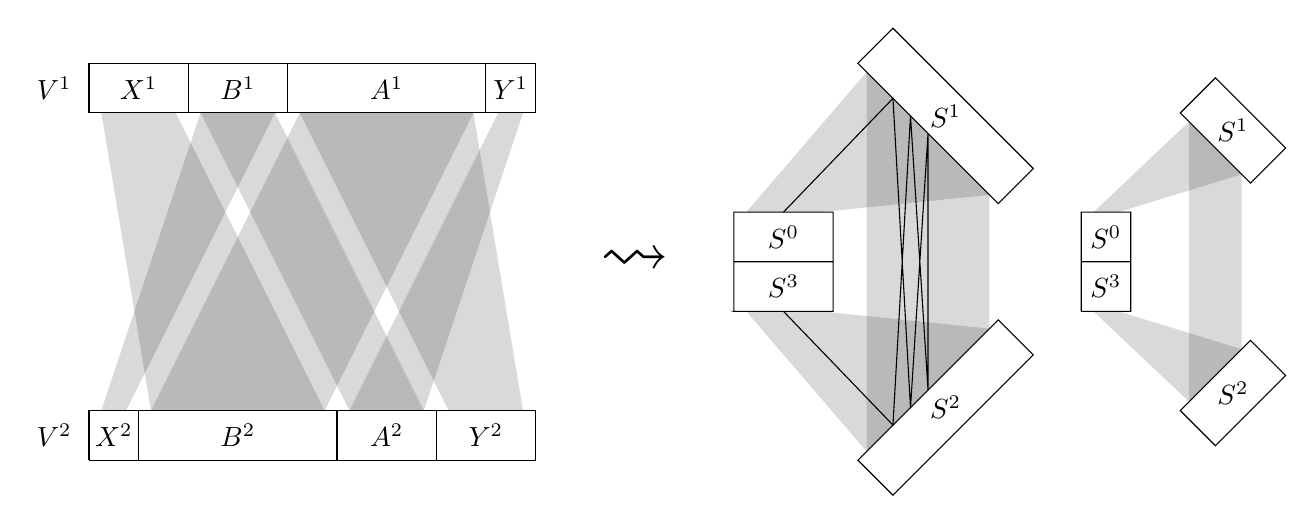
\begin{tikzpicture}[scale=0.63]

\def\y{0}
\def\h{1}
\draw (0,\y) -| (9,1+\y) -| (8,\y)
      (8,1+\y) -| (4,\y)
      (4,1+\y) -| (2,\y)
      (2,1+\y) -| (0,\y);

\node at (-0.7,0.5+\y) {$V^\h$};
\node at (1,0.5+\y) {$X^\h$};
\node at (3,0.5+\y) {$B^\h$};
\node at (6,0.5+\y) {$A^\h$};
\node at (8.5,0.5+\y) {$Y^\h$};

\def\y{-7}
\def\h{2}
\draw (0,\y) -| (9,1+\y) -| (7,\y)
      (7,1+\y) -| (5,\y)
      (5,1+\y) -| (1,\y)
      (1,1+\y) -| (0,\y);

\node at (-0.7,0.5+\y) {$V^\h$};
\node at (0.5,0.5+\y) {$X^\h$};
\node at (3,0.5+\y) {$B^\h$};
\node at (6,0.5+\y) {$A^\h$};
\node at (8,0.5+\y) {$Y^\h$};

\fill [opacity=0.15] (0.25,0) -- (1.75,0) -- (4.75,1+\y) -- (1.25,1+\y) -- cycle;
\fill [opacity=0.15] (2.25,0) -- (3.75,0) -- (0.75,1+\y) -- (0.25,1+\y) -- cycle;
\fill [opacity=0.15] (4.25,0) -- (7.75,0) -- (4.75,1+\y) -- (1.25,1+\y) -- cycle;
\fill [opacity=0.15] (2.25,0) -- (3.75,0) -- (6.75,1+\y) -- (5.25,1+\y) -- cycle;
\fill [opacity=0.15] (4.25,0) -- (7.75,0) -- (8.75,1+\y) -- (7.25,1+\y) -- cycle;
\fill [opacity=0.15] (8.25,0) -- (8.75,0) -- (6.75,1+\y) -- (5.25,1+\y) -- cycle;

\def\sqrt{1.41421356237}

\def\x{13}

\def\y{-3}
\draw (\x,\y-1) -| (\x+2,\y+1) -| cycle
      (\x,\y) -- (\x+2,\y);
\draw (\x+2.5,\y+4) -- (\x+2.5+1/\sqrt,\y+4+1/\sqrt) -- (\x+2.5+5/\sqrt,\y+4-3/\sqrt) -- (\x+2.5+4/\sqrt,\y+4-4/\sqrt) -- cycle;

\draw (\x+2.5,\y-4) -- (\x+2.5+1/\sqrt,\y-4-1/\sqrt) -- (\x+2.5+5/\sqrt,\y-4+3/\sqrt) -- (\x+2.5+4/\sqrt,\y-4+4/\sqrt) -- cycle;

\fill [opacity=0.15] (\x+0.25,\y-1) -- (\x+1.75,\y-1) -- (\x+2.5+3.75/\sqrt,\y-4+3.75/\sqrt) -- (\x+2.5+0.25/\sqrt,\y-4+0.25/\sqrt) -- cycle;
\fill [opacity=0.15] (\x+0.25,\y+1) -- (\x+1.75,\y+1) -- (\x+2.5+3.75/\sqrt,\y+4-3.75/\sqrt) -- (\x+2.5+0.25/\sqrt,\y+4-0.25/\sqrt) -- cycle;

\fill [opacity=0.15] (\x+2.5+3.75/\sqrt,\y-4+3.75/\sqrt) -- (\x+2.5+0.25/\sqrt,\y-4+0.25/\sqrt) -- (\x+2.5+0.25/\sqrt,\y+4-0.25/\sqrt) -- (\x+2.5+3.75/\sqrt,\y+4-3.75/\sqrt) -- cycle;

\draw (\x+1,\y-1) -- (\x+2.5+1/\sqrt,\y-4+1/\sqrt) -- (\x+2.5+1.5/\sqrt,\y+4-1.5/\sqrt) -- (\x+2.5+2/\sqrt,\y-4+2/\sqrt) -- (\x+2.5+2/\sqrt,\y+4-2/\sqrt) -- (\x+2.5+1.5/\sqrt,\y-4+1.5/\sqrt) -- (\x+2.5+1/\sqrt,\y+4-1/\sqrt) -- (\x+1,\y+1);

\node at (\x+1,\y+0.5) {$S^0$};
\node at (\x+1,\y-0.5) {$S^3$};
\node at (\x+2.5+2.5/\sqrt,\y+4-1.5/\sqrt) {$S^1$};
\node at (\x+2.5+2.5/\sqrt,\y-4+1.5/\sqrt) {$S^2$};

\def\x{19}
\def\y{-3}
\def\sqrt{1.41421356237}
\draw (\x+1,\y-1) -| (\x+2,\y+1) -| cycle
      (\x+1,\y) -- (\x+2,\y);
\draw (\x+3,\y+3) -- (\x+3+1/\sqrt,\y+3+1/\sqrt) -- (\x+3+3/\sqrt,\y+3-1/\sqrt) -- (\x+3+2/\sqrt,\y+3-2/\sqrt) -- cycle;

\draw (\x+3,\y-3) -- (\x+3+1/\sqrt,\y-3-1/\sqrt) -- (\x+3+3/\sqrt,\y-3+1/\sqrt) -- (\x+3+2/\sqrt,\y-3+2/\sqrt) -- cycle;

\fill [opacity=0.15] (\x+1.25,\y-1) -- (\x+1.75,\y-1) -- (\x+3+1.75/\sqrt,\y-3+1.75/\sqrt) -- (\x+3+0.25/\sqrt,\y-3+0.25/\sqrt) -- cycle;
\fill [opacity=0.15] (\x+1.25,\y+1) -- (\x+1.75,\y+1) -- (\x+3+1.75/\sqrt,\y+3-1.75/\sqrt) -- (\x+3+0.25/\sqrt,\y+3-0.25/\sqrt) -- cycle;

\fill [opacity=0.15] (\x+3+1.75/\sqrt,\y-3+1.75/\sqrt) -- (\x+3+0.25/\sqrt,\y-3+0.25/\sqrt) -- (\x+3+0.25/\sqrt,\y+3-0.25/\sqrt) -- (\x+3+1.75/\sqrt,\y+3-1.75/\sqrt) -- cycle;

\node at (\x+1.5,\y+0.5) {$S^0$};
\node at (\x+1.5,\y-0.5) {$S^3$};
\node at (\x+3+1.5/\sqrt,\y+3-0.5/\sqrt) {$S^1$};
\node at (\x+3+1.5/\sqrt,\y-3+0.5/\sqrt) {$S^2$};

\node [font=\Huge] at (11,-3) {$\rightsquigarrow$};

\end{tikzpicture}
\end{center}

\protect\caption{\label{fig:cluster-paths}From super-regular pairs to cluster-cycles.
An example special path is shown, for $k=7$.}
\end{figure}



\section{Concluding Remarks}

We have proved that any given bounded-degree spanning tree typically
appears when a linear number of random edges are added to a dense
graph. There are a few interesting questions that remain open. Most
prominent is the question of embedding more general kinds of spanning
subgraphs into randomly perturbed graphs. It would be particularly
interesting if the general result of \cite{BST09} (concerning arbitrary
spanning graphs with bounded degree and low bandwidth) could be adapted
to this setting. It is also possible that our use of Szemer\'edi's
regularity lemma could be avoided, thus drastically improving the
constants $\c\left(\a\right)$ and perhaps allowing us to say something
about random perturbations of graphs which have slightly sublinear
minimum degree.

\noindent \textbf{Acknowledgement.} Parts of this work were carried
out when the first author visited the Institute for Mathematical Research
(FIM) of ETH Zurich, and also when the third author visited the School
of Mathematical Sciences of Tel Aviv University, Israel. We would
like to thank both institutions for their hospitality and for creating
a stimulating research environment.

\bibliographystyle{amsplain_initials}
\bibliography{references}

\end{document}
